\chapter{Synchronisation}

\section{Signale}
\begin{description}
\item[Synchronisation (hier)] Dafür sorgen, dass gewisse Abläufe ausgeschlossen sind.\\
Auch: Koordination.
\item[Signal (auch: Handshake, Meldung, engl. notification)] Hinweis an einen anderen Thread, dass er weitermachen kann.
\end{description}

Analogie:
\begin{itemize}
	\item Startschuss beim Wettlauf
	\item Staffel beim Staffellauf
	\item Anschlusszug muss warten
	\item Becher vor Kaffeezulauf
\end{itemize}

Ein Signal kann durch eine Sperre implementiert werden: 
\begin{itemize}
	\item signalisieren (auch: melden) = freigeben
	\item warten = belegen
\end{itemize}
Das Signal soll garantieren, dass eine gewisse Reihenfolge eingehalten wird.\\
\\ % TODO: Einrücken
P1: S1;
	freigeben(l);
P2:	belegen(l);
	S2;\\
% TODO: Grafik 20160519_SynchronisationZeitstrahl einfügen
\\
l muss freigegeben worden sein, bevor es wieder belegt werden kann, also findet S1 vor S2 statt.\\
\\
Durch die Verwendung von Signalen schränkt man die Menge der Abläufe ein.\\
Nachteil: weniger Parallelität\\
Extremfall: Nur noch eine Reihenfolge möglich; der Ablauf wird seriell. Abgesehen vom Koordinationsaufwand zu einem seriellen Programm gleichwertig.

\section[Beispiel: Erzeuger/Verbraucher (1)]{Beispiel: Erzeuger/Verbraucher-Problem, 1. Version}
Erzeuger und Verbraucher sind Threads. Der Erzeuger erzeugt Datenblöcke. Der Verbraucher holt die Datenblöcke ab und verarbeitet sie.\\
Die erzeugten aber noch nicht verbrauchten Datenblöcke werden in einem Puffer (:= Warteschlange) zwischengespeichert.\\
\\
\textbf{1. Version}: 1 Erzeuger, 1 Verbraucher, Puffer für 1 Datenblock.\\
\\ % TODO: Pseudocode
Thread erz:
	Wiederhole
		herstellen(datenblock);
		einreihen(puffer, datenblock);
Thread verbr:
	Wiederhole
		abholen(puffer, datenblock);
		verarbeiten(datenblock);\\
\\
Prozedur einreihen(puffer, datenblock):
\begin{enumerate}
	\item belegen(leer);
	\item kopieren(datenblock, puffer); -> kopiert Datenblock in Puffer
	\item freigeben(voll);
\end{enumerate}
Prozedur abholen(puffer, datenblock):
\begin{enumerate}
	\setcounter{enumi}{3}
	\item belegen(voll);
	\item kopieren(puffer, datenblock); -> kopiert Puffer in Datenblock
\end{enumerate}
Hauptprogramm (HP):
\begin{enumerate}
	\item[] Sperre voll anlegen; -> als belegt
	\item[] Sperre leer anlegen; -> als belegt
	\item[] Threads erz und verbr anlegen und laufen lassen;
	\item[0.] freigeben(leer);
\end{enumerate}

\subsubsection*{Kausalitätsgraph:}
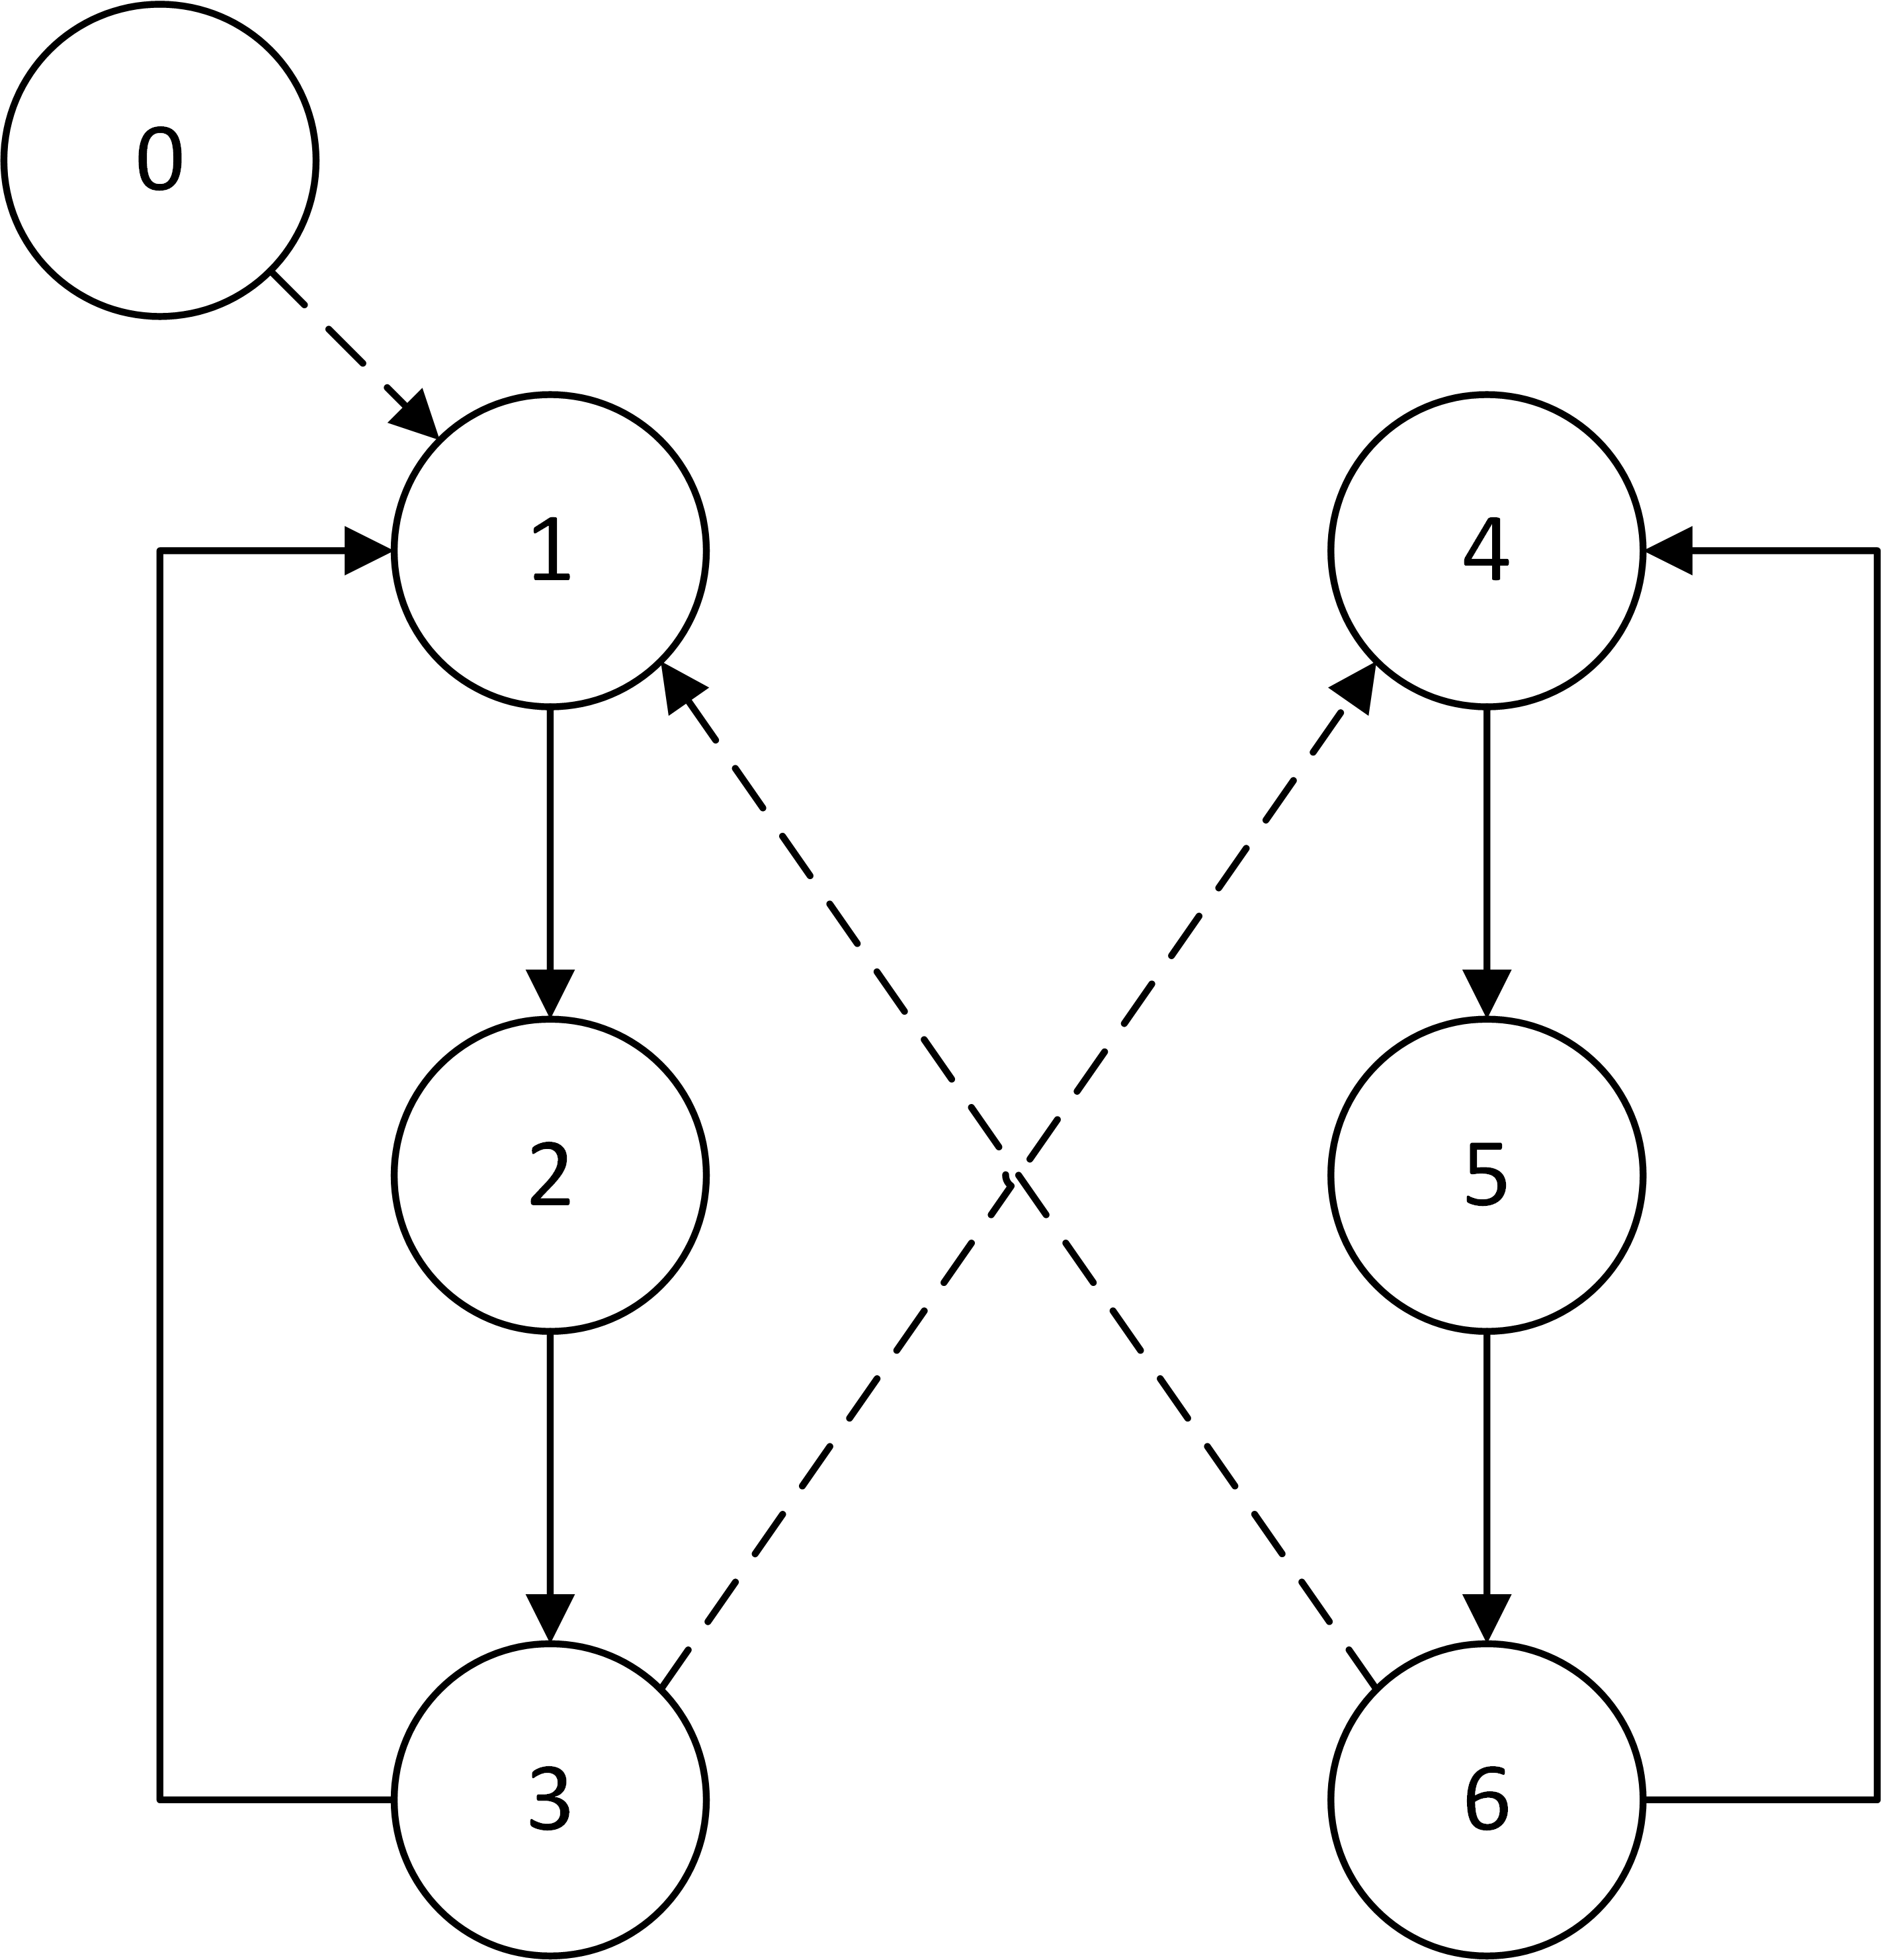
\includegraphics[width=.4\textwidth]{SynchronisationKausalitaetsgraph}

% Pfeil
Programmreihenfolge
% Gestrichelter Pfeil
Reihenfolge erzwungen durch Signal

\subsubsection*{Petri-Netz:} % TODO: Grafik Petrinetz
Legende für Petri-Netz: Kreis Platz, Strich Transition, Punkt Token.\\
\\
Bipartiter Graph: Zwei Sorten von Knoten; Pfeile nur zwischen verschiedenen Knoten-Sorten.
% TODO: Wenn möglich, Petrinetz laufen lassen

\section{Semaphore}

\section[Beispiel: Erzeuger/Verbraucher (2)]{Beispiel: Erzeuger/Verbraucher-Problem, 2. Version}

\section{Bedingte kritische Bereiche}

\section[Beispiel: Erzeuger/Verbraucher (3)]{Beispiel: Erzeuger/Verbraucher-Problem, 3. Version}

\section{Wiederbetretbare Sperren}

\section{Leser/Schreiber-Problem}